\documentclass[../../main.tex]{subfiles}
\begin{document}
\graphicspath{{./figures}}
\chapter{Integración con GNU Radio}
El \textit{core} de adquisición y preprocesamiento desarrollado en la CIAA-ACC empaqueta y envía los datos de los 16 canales preprocesados por un \textit{socket} UDP de acuerdo al software que corre dentro del PS desarrollado en \cite{proyecto-jose}. Por otro lado, en \cite{proyecto-grigo} se desarrollaron bloques en GNU Radio para detectar DoA y realizar la conformación digital de haz. En este capítulo se busca desarrollar un puente entre estos dos proyectos para lograr integrarlos.

\section{Flujo de trabajo en GNU Radio}
Como se comentó en la sección \ref{sec::procesamiento-externo}, GNU Radio es un software para el desarrollo de SDR \cite{GNURadio}. El mismo consiste de una librería desarrollada parte en C++ y parte en Python. Cuenta además con una interfaz de usuario que provee una forma sencilla de desarrollo de tipo \textit{low code} mediante bloques. Cuando se elige este enfoque de desarrollo, GNU Radio luego se encarga de escribir en código de C++ o Python la configuración expresada mediante el diagrama de bloques. Esto resulta útil ya que le permite al usuario modificar el código generado según le sea conveniente.

Un ejemplo del desarrollo con bloques y la GUI resultante generada por la librería se muestra en la figura \ref{fig::gnu-dummy} donde se genera  y se grafica una señal cosenoidal.\unsure{existe esta palabra?} Para esto se usan 3 bloques: 
\begin{itemize}
    \item \textit{Signal Source}: genera una señal. Puede configurarse qué tipo de señal, su frecuencia, su amplitud, entre otros.
    \item \textit{Throttle}: limita la cantidad de muestras por segundo que se procesan. Esto resulta útil para controlar la cantidad de recursos utilizados por el \textit{framework}.
    \item \textit{QT GUI Time Sink}: Genera un elemento de GUI que grafica en tiempo real la amplitud de la señal recibida en función del tiempo.
\end{itemize}

Además de los bloques incluidos con la librería como los recién mencionados, el \textit{framework} también permite la creación de bloques personalizados por parte del usuario mediante la herramienta \textit{gr\_modtool} \cite{gr-modtool}. Estos bloques reciben el nombre de \textit{Out of Tree Module} (módulo OOT) y permiten extender las funcionalidades básicas del \textit{framework} haciendo posible también la incorporación de bloques desarrollados por otros usuarios.

\begin{figure}[H]
    \centering
    \subcaptionbox{Diagrama de bloques implementado en GNU Radio.\label{fig::gnu-dummy-bd}}
    {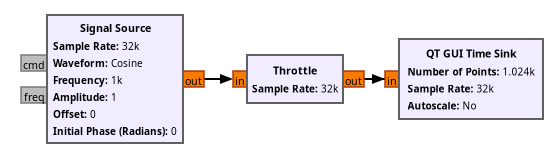
\includegraphics[width=0.5\linewidth]{gnu-dummy-bd.png}}\\[1PC]
    \subcaptionbox{GUI generada por GNU Radio.\label{fig::gnu-dummy-plot}}
    {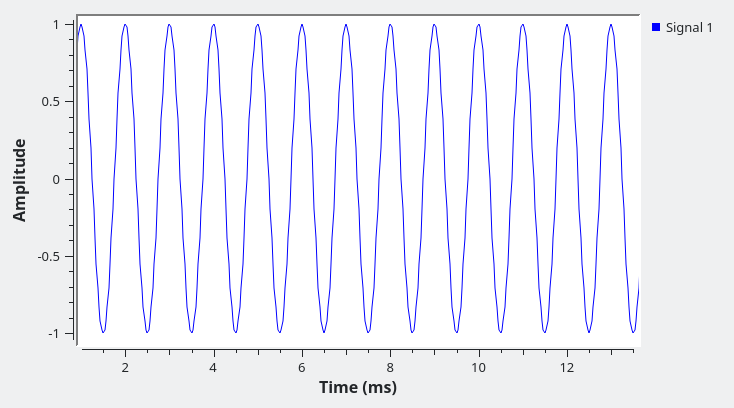
\includegraphics[width=0.5\linewidth]{gnu-dummy-plot.png}}
    \caption{Diagrama de bloques sencillo implementado en GNU Radio y la interfaz generada por el mismo.}
    \label{fig::gnu-dummy}
\end{figure}

\section{Recepción con GNU Radio}
\todo{Poner tabla con bloques nativos utilizados y otra con bloques custom o de otros usuarios (parecido a lo que hicimos con las IPs en el preproc)}
\subsection{Comunicación entre CIAA-ACC y GNU Radio}
Se mencionó anteriormente que el sistema de adquisición y preprocesamiento envía paquetes con los datos adquiridos mediante un socket UDP. Luego, del lado de GNU Radio, esos paquetes deben capturarse e interpretarse correctamente. 

La captura de los paquetes puede lograrse a través de la instanciación del bloque \texttt{UDP Source}\todo{ref}, disponible con la instalación de la librería. Este bloque escucha el tráfico UDP entrante a un dado puerto y proveniente de una dirección IP \unsure{Acá IP es Internet Protocol, no es Intellectual Property, cómo se resuelve esto?} determinada. De esta forma, configurándolo con la dirección IP de la CIAA-ACC y el número de puerto al que la placa transmite, pueden recibirse los datos exitósamente en GNU Radio. 

Al configurar el bloque \texttt{UDP Source} también hay que especificarle el tamaño de paquete que esperamos recibir. Resulta importante notar que, a diferencia de la mayoría de los bloques de la librería, dicho tamaño se escribe siempre en bytes, independientemente del tipo de dato con el que se esté trabajando.

Por otro lado, para lograr una correcta interpretación de los datos debe tenerse en cuenta el tipo de dato que se está adquiriendo. El sistema de tipado de la librería se desarrolla en el apéndice \ref{ap::tipado-gnu}. En el caso de este proyecto, los datos que llegan desde el sistema de adquisición y preprocesamiento son complejos, donde la parte real y la imaginaria se componen de 16 bits cada una. \todo{ref} El bloque \texttt{UDP Source}, sin embargo, no es capaz, por defecto, de entregar los datos en este formato, ya que el tipo complejo con el que trabaja (\texttt{Complex Float 32}) se compone de 64 bits en total.

Una solución a este problema es leer los datos de a 16 bits y luego agrupar dos datos de 16 bits como un único dato complejo de 32 bits. Esto se logra configurando el tipo de dato del \texttt{UDP Source} como \texttt{short}, que es un entero de 16 bits. Luego mediante la instanciación del bloque \texttt{IShort To Complex}, el cual forma parte de la librería, se convierten dos \texttt{shorts} consecutivos en un \texttt{Complex Float 32}. De esta manera, se puede trabajar durante todo el procesamiento con datos del tipo \texttt{Complex Float 32}.

\subsection{Lector de \textit{header}}
El paquete enviado por la placa incorpora un \textit{header}. El mismo fue desarrollado en \cite{proyecto-jose} y su estructura puede encontrarse en \texttt{PIQuinteros/SoftwarePS/client/lib/acqPack.h}.

Este encabezado consiste de 88 bytes y contiene, entre otras cosas, las \textit{fifo flags}. Estas son señales de control que permiten el monitoreo de las FIFOs dentro de la FPGA. Resultan relevantes para detectar por ejemplo situaciones de \textit{overflow}, lo cual puede ocurrir si las FIFOs se llenan antes de ser leídas por el PS.

Para poder decodificar el encabezado de los paquetes se implementó un módulo OOT personalizado en GNU Radio empleando la herramienta \textit{gr\_modtool} mencionada anteriormente. La definición del mismo se encuentra en \texttt{GNU-Radio/OOT/gr-beamforming/lib/HeaderReader\_impl.h}. 

El bloque recibe un vector del tamaño del \textit{header} (88 bytes) y lo decodifica. A continuación verifica que la información relevante durante ejecución como la \textit{flag} de \textit{FIFO overflow} y la \textit{flag} de \textit{FIFO full} sea la adecuada y, en caso contrario, avisa al usuario escribiéndolo a la consola integrada de GNU Radio.

\todo{Poner foto del header o referencia si es que lo expliqué antes. Ver pag 70 del informe de José}

\subsection{Comprobación de funcionamiento}
Para corroborar que la comunicación entre la placa y el SDR estaba funcionando de manera correcta se configuró la FPGA para obtener datos del contador de debug mediante la escritura de los registros \todo{decir registros, poner ref a cuando se explicó}. A continuación se disparó una captura de datos, la cual se adquirió con GNU Radio.

En la figura \ref{fig::gnu-simplificado} se muestra el esquemático utilizado para esta comprobación. El mismo incorpora lo anteriormente discutido junto con dos puntos de visualización donde se colocaron instancias del bloque \texttt{QT GUI Sink}, el cual brinda, entre otras cosas un gráfico en tiempo y en frecuencia de la señal de entrada.

Se separaron los datos en \textit{header} y \textit{payload}

\figura{gnu-simplificado}{Esquemático utilizado para la prueba de comunicación entre la CIAA-ACC y GNU Radio.}




\section{Algoritmos de \textit{beamforming}}
\subsection{Verificación de bloques previamente desarrollados}
\subsection{Implementación de bloque propio de BF}

\section{Algoritmos de seguimiento de señal}
\subsection{Verificación de algoritmo de DoA}
\subsection{Implementación de seguimiento mediante TLEs}
\subsubsection{Librería orbit-predictor}

\section{Efecto Doppler}
%comentar y mostrar gráficos
\subsection{Corrección mediante TLEs}

\section{Tests? Screenshots de las cosas andando?}

\end{document}